\subsection{比例}\label{subsec:czjh2-6-1}

\begin{enhancedline}

前面,我们学习了全等图形。两个全等图形的形状相同,大小也相同,它们能够完全重合。
我们还常见到这样的一些图形,如国旗上的大五角星和小五角星;
图 \ref{fig:czjh2-6-1} 中我们伟大祖国的两幅大小不同的地图。
这些图形大小虽然不同,但形状却是相同的。

\begin{figure}[htbp]
    \centering
    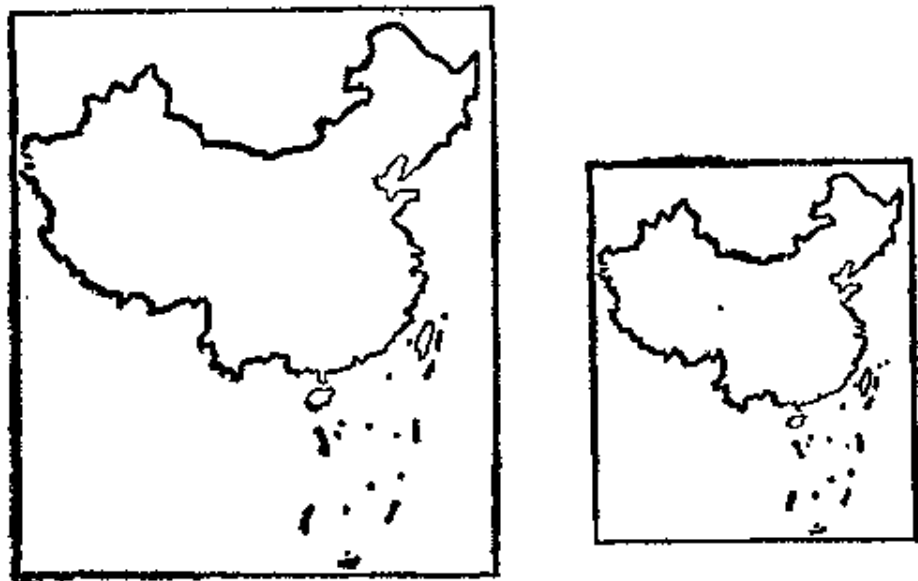
\includegraphics[width=5cm]{../pic/czjh2-ch6-01.png}
    \caption{}\label{fig:czjh2-6-1}
\end{figure}

为了研究这些形状相同的图形之间的关系,我们需要先研究比例和比例线段。

在小学里,我们学过比例,就是两个比相等的式子。如
\begin{gather*}
    \exdfrac{80}{2} = \exdfrac{240}{6} \quad \text{或} \quad 80:2 = 240:6 \juhao
\end{gather*}

%\qquad $\dfrac{80}{2} = \dfrac{240}{6}$ 或 $80:2 = 240:6$。

如果用字母來表示数,那么比例可以写成如下的形式(只研究所有的字母都不等于零的情形):
\begin{gather*}
    \exdfrac{a}{b} = \exdfrac{c}{d} \quad \text{或} \quad a:b = c:d \juhao
\end{gather*}

在比例中,$a$、$d$ 叫做\zhongdian{比例外项},
$b$、$c$ 叫做\zhongdian{比例内项},
$d$ 叫做 $a$、$b$、$c$ 的\zhongdian{第四比例项}。
如果比例中两个比例内项相等,即比例为
\begin{gather*}
    \exdfrac{a}{b} = \exdfrac{b}{c} \quad \text{或} \quad a:b = b:c
\end{gather*}
时,我们把 $b$ 叫做 $a$ 和 $c$ 的\zhongdian{比例中项}。

在比例 $\exdfrac{a}{b} = \exdfrac{c}{d}$ 的两边同乘以 $bd$,得到
\begin{gather*}
    ad = bc \juhao
\end{gather*}

这个推理步骤就是:

$\because$ \quad $\exdfrac{a}{b} = \exdfrac{c}{d}$,

$\therefore$ \quad $ad = bc$。

为了简明,可以把这个推理步骤写成:
\begin{gather}
    \exdfrac{a}{b} = \exdfrac{c}{d} \tuichu  ad = bc \juhao  \tag{1}
\end{gather}

符号 “$\tuichu$” 读作 “推出”。

在等式 $ad = bc$  的两边同除以 $bd$,又得到 $\exdfrac{a}{b} = \exdfrac{c}{d}$,即
\begin{gather}
    ad = bc  \tuichu  \exdfrac{a}{b} = \exdfrac{c}{d} \juhao  \tag{2}
\end{gather}

(1)、(2) 式合起来表示 $\exdfrac{a}{b} = \exdfrac{c}{d}$ 与 $ad = bc$ 可以
互相推出,这是比例的基本性质。

\begin{dingli}[比例的性质定理]
    $$ \bm{
        \exdfrac{a}{b} = \exdfrac{c}{d} \dengjiayu ad = bc \juhao
    }$$
\end{dingli}

符号 “$\dengjiayu$” 读作“等价于”。它表示从左端可以推出右端,并且从右端也可以推出左端。

\begin{tuilun}[推论]
    $\bm{
        \exdfrac{a}{b} = \exdfrac{b}{c}  \dengjiayu  b^2 = ac \juhao
    }$
\end{tuilun}

根据比例的性质定理,一个比例可以得出多种不同的比例变形。例如,

$\exdfrac{a}{b} = \exdfrac{c}{d}  \tuichu  ad = bc  \tuichu  bc = ad   \tuichu \exdfrac{b}{a} = \exdfrac{d}{c}$。

由于  $ad = bc$ 可以写成  $bc = ad$, $ad = cb$, $cb = da$,… 等七种形式,
所以由 $\exdfrac{a}{b} = \exdfrac{c}{d}$ 又可以得出
$\exdfrac{b}{a} = \exdfrac{d}{c}$,
$\exdfrac{a}{c} = \exdfrac{b}{d}$,
$\exdfrac{c}{d} = \exdfrac{a}{b}$,… 等七种不同形式。

\liti 依据下列各式,求 $a:b$ :

(1)$3a = 4b$;(2)$\exdfrac{a}{5} = \exdfrac{b}{7}$。

\jie (1)$3a = 4b  \tuichu \exdfrac{a}{b} = \exdfrac{4}{3}$;

(2)$\exdfrac{a}{5} = \exdfrac{b}{7}  \tuichu  \exdfrac{a}{b} = \exdfrac{5}{7}$。


下面,我们再学习比例的两个重要性质:

1. \begin{xingzhi}[合比性质]
    \newline\ \hspace*{3em}
    $\bm{
        \exdfrac{a}{b} = \exdfrac{c}{d}  \tuichu \dfrac{a \pm b}{b} = \dfrac{c \pm d}{d} \juhao
    }$
\end{xingzhi}

\zhengming $\begin{aligned}[t]
    \exdfrac{a}{b} = \exdfrac{c}{d}  &\tuichu  \exdfrac{a}{b} \pm 1 = \exdfrac{c}{d} \pm 1 \\
                                     &\tuichu  \dfrac{a \pm b}{b} = \dfrac{c \pm d}{d} \juhao
\end{aligned}$


2. \begin{xingzhi}[等比性质]
    \newline\ \hspace*{3em}
    $\begin{aligned}[t]
        \bm{\exdfrac{a}{b}} &= \bm{\exdfrac{c}{d} = \cdots = \exdfrac{m}{n} \; (b + d + \cdots + n \neq 0)} \\
                            & \bm{\tuichu \dfrac{a  + c + \cdots + m}{b + d + \cdots + n} = \exdfrac{a}{b} \juhao}
    \end{aligned}$
\end{xingzhi}

\zhengming 设 $\exdfrac{a}{b} = \exdfrac{c}{d} = \cdots = \exdfrac{m}{n} = k$,
那么 $a = bk$, $c = dk$,…, $m = nk$。

$\begin{aligned}[t]
    \dfrac{a + c + \cdots + m}{b + d + \cdots + n}
        &= \dfrac{bk + dk + \cdots + nk}{b + d + \cdots + n} \\
        &= \dfrac{(b + d + \cdots + n)k}{b + d + \cdots + n} = k = \exdfrac{a}{b} \juhao
\end{aligned}$



\liti (1)已知: $\dfrac{a - b}{b} = \exdfrac{3}{8}$。求证  $\exdfrac{a}{b} = \dfrac{11}{8}$;

(2)已知: $\exdfrac{a}{b} = \exdfrac{c}{d} \; (b \pm d \neq 0)$。
求证: $\dfrac{a + c}{a - c} = \dfrac{b + d}{b - d}$。

\zhengming (1) $\begin{aligned}[t]
    \dfrac{a - b}{b} = \exdfrac{3}{8}
        &\tuichu \dfrac{a - b + b}{8} = \dfrac{3 + 8}{8} \\
        &\tuichu \exdfrac{a}{b} = \dfrac{11}{8} \fenhao
\end{aligned}$


(2)$\begin{aligned}[t]
    \exdfrac{a}{b} = \exdfrac{c}{d}
        &\tuichu \left\{
                \begin{gathered}
                    \dfrac{a + c}{b + d} = \exdfrac{a}{b} \\
                    \dfrac{a - c}{b - d} = \exdfrac{a}{b} \\
                \end{gathered}
            \right\} \tuichu \dfrac{a + c}{b + d} = \dfrac{a - c}{b - d} \\
        &\tuichu \dfrac{a + c}{a - c} = \dfrac{b + d}{b - d} \juhao
\end{aligned}$


\liti 已知: $\exdfrac{a}{b}  = \exdfrac{c}{d} = \exdfrac{e}{f} = 3$,
$b + d + f = 4$。 求 $a + c + e$。

\jie $\begin{aligned}[t]
    \exdfrac{a}{b}  = \exdfrac{c}{d} = \exdfrac{e}{f} = 3
        & \tuichu \dfrac{a + c + e}{b + d + f} = 3 \\
        & \left.\begin{aligned}
                \tuichu a + c + e = 3 (b + d + f) & \\
                b + d + f = 4 &
            \end{aligned} \right\} \\
        & \tuichu a + c + e = 3 \times 4 = 12 \juhao
\end{aligned}$


\begin{lianxi}

\xiaoti{求下列各式中的 $x$:}
\begin{xiaoxiaotis}

    \begin{tblr}{columns={18em, colsep=0pt}}
        \xxt{$4:x = 3:5$;}  & \xxt{$(x + 2):x = 11:9$;} \\
        \xxt{$3:x = x:12$;} & \xxt{$1:x = x:(1 - x)$。}
    \end{tblr}

\end{xiaoxiaotis}


\xiaoti{已知: $\exdfrac{a}{b} = \exdfrac{c}{d}$。写出其他七个比例式,并指出其中
    哪些是以 $a$ 和 $d$ 为外项,以 $b$ 和 $c$ 为内项的比例式,
    哪些是以 $b$ 和 $c$ 为外项,以 $a$ 和 $d$ 为内项的比例式。
}


\xiaoti{从下列各式求 $x:y$:}
\begin{xiaoxiaotis}

    \begin{tblr}{columns={12em, colsep=0pt}}
        \xxt{$3y = 4x$;} & \xxt{$3:2 = y:x$;} & \xxt{$7:x = 4:y$;} \\
        \xxt{$m:y = n:x$;} & \xxt{$(x+y):y = 8:3$;} & \xxt{$(x-y):y = 1:2$。}
    \end{tblr}

\end{xiaoxiaotis}


\xiaoti{已知 $h$ 是 $e$、$f$、$g$ 的第四比例项,写出比例式。}

\xiaoti{已知: $\exdfrac{a}{b} = \exdfrac{c}{d} = \exdfrac{e}{f} = \exdfrac{5}{7}$。
    求 $\dfrac{2a - c + 7e}{2b - d + 7f}$。
}


\xiaoti{(口答)}
\begin{xiaoxiaotis}

    \xxt{$\exdfrac{a}{b}$ 是不是等于 $\exdfrac{a^2}{b^2}$? 为什么?}

    \xxt{从 $\exdfrac{a}{b} = \exdfrac{c}{d}$ 能不能得出 $\exdfrac{a^2}{b^2} = \exdfrac{c^2}{d^2}$?为什么?}

\end{xiaoxiaotis}


\xiaoti{从下面两个比例可以推出什么结果:}
\begin{xiaoxiaotis}

    \xxt{$b:a = c:b$;}

    \xxt{$b:a = b:c$。}

\end{xiaoxiaotis}

\end{lianxi}
\end{enhancedline}

